\documentclass{article}
\usepackage[utf8]{inputenc}
\usepackage{blkarray}
\usepackage{amsthm}
\usepackage{amsfonts}
\usepackage{amsmath}
\usepackage{enumitem}
\usepackage{amssymb}
\usepackage{graphicx}
\usepackage[utf8]{inputenc}
\usepackage[margin=1in]{geometry}
\usepackage{parskip}
\usepackage{graphicx}
\usepackage{media9}
\usepackage{multimedia}
 \graphicspath{ {./images/} }

\title{Markov Chains \&\ Musical Algorithms}
\author{Rahul Prasad and Saman de Silva}
\date{December 2022}

\begin{document}
\maketitle

\section{Introduction}

Making music is a difficult task. We wanted to see if we could find an application of linear algebra to allow us to generate music in a controlled, yet random way. 

We decided to use Markov Chains as the basis for this task, moving between elements of a musical melody using Markov Chains. They allow us to assign probabilities while not being completely random, an important aspect of generating melodies. It's difficult to create a strong computer-generated music generator because of the amount of patterns that appear in melodies, and the delicate balance of pattern and randomness that gives every melody its own unique sound.

So, for this paper, our ultimate goal was to research Markov Chains, and apply them to generating music. We studied previous attempts at this task as well as developing our own method to do so. 

For our purposes, we wanted to just create a string of notes that have some musical significance -- rhythm is out of the scope of this paper (which we will talk about later on).

We will begin by introducing Markov Chains.

\section{Understanding Markov Chains}

\textbf{Markov Chains} are at the crux of our analysis in this paper. It forces us to use linear algebra and matrices to analyze data from a different lens. Rather than see matrices as a system of linear equations, we can view them as encoding valuable data on the probability of existing in some \textit{state}. To begin, we'll examine some definitions in context.

\setlength{\parskip}{10pt}

\begin{enumerate}[label=]
    \item \textbf{Definition.} A probability vector is a vector of non-negative values that sum to one. 
\end{enumerate}

\setlength{\parskip}{15pt}

\noindent Note that probability vectors can be vertical or horizontal. For our purposes, we will be considering vertical probability vectors.

\setlength{\parskip}{10pt}

\begin{enumerate}[label=]
    \item \textbf{Definition.} A state vector is a probability vector that describes the state of an object.
\end{enumerate}

\setlength{\parskip}{10pt}

\noindent Consider the following state vectors:

\begin{center}
    $A_1=\begin{bmatrix} 1\\0\\0\end{bmatrix}$, $A_2=\begin{bmatrix}.6\\.3\\.1\end{bmatrix}$.
\end{center}

\noindent These vectors represent a \textbf{set} of probabilities that describe the \textbf{state} of an object. So, 
\begin{itemize}
    \setlength\itemsep{-1em}
    \item $A_1$ describes that the object has a $100\%$ chance of existing as state one,
    \item $A_2$ describes that the object has $60\%$ of existing as state one, a $30\%$ chance of existing as state two, and a $10\%$ chance of existing as state three.
\end{itemize}
    
\noindent Probability vectors can be combined to form the columns of an $n \times n$ stochastic matrix.

\setlength{\parskip}{15pt}

\begin{enumerate}[label=]
    \item \textbf{Definition.} A stochastic matrix is a square matrix of non-negative values with columns that sum to one.
\end{enumerate}

\setlength{\parskip}{10pt}

\noindent Consider the $3 \times 3$ stochastic matrix $A$:

\begin{center}
    $A=
    \begin{bmatrix} .7&.3&.9\\.2&.1&0\\.1&.6&.1\\ \end{bmatrix}$
\end{center}

\noindent Note that each column still has the sum 1.

\begin{enumerate}[label=]
    \item \textbf{Definition.} A Markov chain is a dynamical system with each state defined by a state vector which evolves according to a difference equation: 

    \begin{align*}
        A&b_n=b_{n+1} \\
        &b\in\mathbb{R}^n
    \end{align*}
\end{enumerate}

Where $A$ is the \textbf{transition matrix} of the chain.

\noindent In Markov Chains, the transition matrix is a stochastic matrix. Suppose there are three arbitrary states for our arbitrary object: A, B and C. 

Recall stochastic matrix $A$ from above:

\begin{center}
    $A=
    \begin{blockarray}{cccc}
    A & B & C \\
        \begin{block}{[ccc]c} 
            .7&.3&.9 & A\\
            .2&.1& 0 & B\\
            .1&.6&.1 & C\\ 
        \end{block}
    \end{blockarray}$
\end{center}

\noindent Each element of the transition matrix made up of vertical probability vectors represents the probability of moving from the \textit{column} label to the corresponding \textit{row} label. For example, 

\begin{enumerate}[label=]
    \setlength\itemsep{-1em}
    \item.7 represents the probability of moving from state $A$ to state $A$; 
    \item.6 represents the probability of moving from state $B$ to state $C$;
    \item \hspace{3pt}0 represents the probability of moving from state $C$ to state $B$.
\end{enumerate}

\noindent Now, as mentioned previously, we can represent the current state of our object with a state vector. Suppose our object begins at state $A$. Thus, its state vector $x$ is

\begin{center}
    $x = \begin{blockarray}{cc}
        \begin{block}{[c]c} 
            1 & A\\
            0 & B\\
            0 & C\\ 
        \end{block}
    \end{blockarray}$
\end{center}

\noindent Where our object has a $100\%$ chance of existing at $A$. Now, we can multiply the state vector and the transition matrix together to yield the resulting state vector after one transition in the chain $x_1$:

\begin{center}
    $x_1 = 
    \begin{blockarray}{ccc}
        \begin{block}{[ccc]} 
            .7&.3&.9\\
            .2&.1& 0\\
            .1&.6&.1\\ 
        \end{block}
    \end{blockarray}
    \begin{blockarray}{c}
        \begin{block}{[c]} 
            1\\
            0\\
            0\\ 
        \end{block}
    \end{blockarray}
    =
    \begin{blockarray}{cc}
        \begin{block}{[c]c} 
            .7 & A\\
            .2 & B\\
            .1 & C\\ 
        \end{block}
    \end{blockarray}
    $
\end{center}

\noindent Thus, our object now has a $70\%$ chance of existing at $A$, $20\%$ chance of existing at $B$, and a $10\%$ chance of existing at $C$. 

Note that $x_1$ is still a probability vector. Is this always true?

\rule{\textwidth}{0.5pt}

A strong property of a Markov Chain (perhaps one of the most fundamental) is its ability to keep a probability vector as an input and an output. Here, we will prove how this works!

\begin{proof} Any stochastic matrix multiplied by a probability vector will yield a probability vector.

Consider $Ax=b$ where A is stochastic and $A \in A_{n\times n}$ as well as $x$ is a probability vector and  $x\in\mathbb{R}^n$. We want to find that $b$ is a probability vector.

\begin{center}
    $\begin{bmatrix}
        a_{11} & \cdots & a_{1n}\\
        \vdots & \ddots & \vdots \\
        a_{n1} & \cdots & a_{nn}
    \end{bmatrix}\begin{bmatrix}
        x_{1} \\ \vdots \\ x_{n}\\
    \end{bmatrix} = \begin{bmatrix}
     a_{11}x_1+\cdots +a_{1n}x_n\\ \vdots \\ a_{n1}x_1+\cdots +a_{nn}x_{n}
    \end{bmatrix}$
\end{center}
    
If we sum the entries of the vector $b$, we get
    \begin{align*}
    (a_{11}x_1+\cdots + a_{1n}x_n)+\cdots+(a_{n1}x_1+\cdots +a_{nn}x_{n})
    \end{align*}

We can then pull out the terms for each degree of $x$ to yield

\begin{align*}
    x_1(a_{11}+\cdots +a_{n1})+\cdots +x_n(a_{1n}+\cdots +a_{nn})
\end{align*}

As we know, this is merely a linear equation of the columns with their components summed. By definition of a stochastic matrix, we know that each column will sum to 1, thus the above equation can be abridged to

\begin{equation*}
    x_1+\cdots +x_{n}=1
\end{equation*}

Therefore, we know that the components of the vector $b$ sum to the value $1$, which therefore proves that $b$ is a probability vector, by its definition.

\end{proof}

\rule{\textwidth}{0.5pt}

Now we know that the product of our transition matrix and a probability vector will always be a probability vector.

\noindent If we then multiply $x_1$ by the transition matrix, we get the state vector of our object after two transitions in the chain $x_2$: 

\begin{center}
    $x_2 = 
    \begin{blockarray}{ccc}
        \begin{block}{[ccc]} 
            .7&.3&.9\\
            .2&.1& 0\\
            .1&.6&.1\\ 
        \end{block}
    \end{blockarray}
    \begin{blockarray}{c}
        \begin{block}{[c]} 
            .7\\
            .2\\
            .1\\ 
        \end{block}
    \end{blockarray}
    =
    \begin{blockarray}{cc}
        \begin{block}{[c]c} 
            .64 & A\\
            .16 & B\\
            .2 & C\\ 
        \end{block}
    \end{blockarray}
    $
\end{center}

\noindent A pattern emerges here: the probability of our object existing at the possible states after $n$ transitions is given by the the state vector $x_n$. We'll come around to calling this vector a \textit{steady-state vector}:

\begin{center}
    $$ \lim_{n\to\infty} x_n = 
    \lim_{n\to\infty}\begin{blockarray}{cccc}
        \begin{block}{[ccc]@{\hphantom{)}}l}
            .7&.3&.9&{\vphantom{)}}^n\\
            .2&.1& 0\\
            .1&.6&.1\\
        \end{block}
    \end{blockarray}
    \begin{blockarray}{c}
        \begin{block}{[c]} 
            .7\\
            .2\\
            .1\\ 
        \end{block}
    \end{blockarray}
    =
    \begin{blockarray}{cc}
        \begin{block}{[c]c} 
            x_{n_1} & A\\
            x_{n_2} & B\\
            x_{n_3} & C\\ 
        \end{block}
    \end{blockarray}
    $$
\end{center}

\begin{enumerate}[label=]
    \item \textbf{Definition.} If $P$ is a stochastic matrix, then $q$ is the steady-state vector for $P$ if and only if $Pq=q$.
\end{enumerate}

This is really fascinating! This means that eigenvalues are encoded into these stochastic matrices and also have a very special meaning. 

As a markov chain is iterated and iterated, it may approach some end behavior, akin to an asymptote. However, this limit can merely be found by computing the eigen space for the given stochastic matrix with the eigen value 1.

As such, we can now relate the steady state vector to a familiar linear algebra concept from class:

\begin{enumerate}[label=]
    \item \textbf{Theorem.} A steady state vector can be found by computing $N(P-I_n)$, then isolating a vector within this space that sums to one.
\end{enumerate}

\rule{\textwidth}{0.5pt}

\begin{proof}
    We know that the steady state vector $q$ of a stochastic matrix $P$ is given by $Pq=q.$ By definition of an eigenvector, $q$ is an eigenvector of $P$ with eigenvalue 1. Thus, $q$ lies in the eigenspace $E_1$ of $P$, given by $E_1=N(P-I_n).$ 

    By definition, $q$ is a probability vector, so the entries of $q$ sum to one. In this instance, we assume that the eigenspace, $E_1$ is a single vector (if not, it doesn't have a steady state). Thus, $q$ will be a vector in $E_1$ such that the entries sum to 1, $\sum_{i}^{n}a_{i1}$.
    
    $q$ is a probability vector by definition, so $q$ is a unique value in the eigenspace where the sum of the entries is 1.
    
\end{proof}
\rule{\textwidth}{0.5pt}

NOTE: not all stochastic matrices will display an end behavior, as parenthetically remarked in the proof. If $\lambda=1$ has a geometric multiplicity that is greater than 1, we know that $dim(E_1)>1$. Or, in other words, $E_1$ will be the span of more than 1 vector, which guts the uniqueness of the probability vector, as there will be multiple instances of a probability vector $q_n$ where the entries of $q_n$ sum to 1 and lie in $E_1$.

We can examine one of these systems here:

\begin{center}
    $A=\begin{blockarray}{cccc}
    A & B & C \\
        \begin{block}{[ccc]c} 
            .7& 0& 0 & A\\
            .25& 0& 1 & B\\
            .05& 1& 0 & C\\ 
        \end{block}
    \end{blockarray}$
\end{center}

In this instance, there is no end state! The matrix will get trapped oscillating between $B$ and $C$ with no resolution, this defines a \textit{periodic} matrix, in that its end behavior will follow some periodic flow. This is a more qualitative way to view the issue, but perhaps easier to digest off of a first glance. We can bring things further into linear algebra with an alternate set of terminology.

An alternate way of thinking about this is by seeing this as a \textit{non-regular} stochastic matrix because any time $A$ is raised to a natural power, it will not contain strictly positive values. Instead, those same zeroes will persist. A matrix that would be strictly positive after being raised to some power - thus, yielding a steady state - is considered a \textit{regular} stochastic matrix.

To summarize,

\begin{enumerate}[label=]
    \item \textbf{Definition.} A stochastic matrix $P$ is regular if and only if $\exists k\in\mathbb{N}$ such that $P^k$ contains strictly positive entries.
\end{enumerate}

\begin{enumerate}[label=]
    \item \textbf{Theorem.} If $P$ is an $n\times n$ regular stochastic matrix, then $P$ has a unique steady-state vector $q$ such that $Pq=q$. Further, if $q_0$ is any initial state and $q_{x+1}=Pq_x$ for all $x\in\mathbb{N}$ then the Markov Chain  converges to $q$ as $x \rightarrow \infty$.

    We'll provide a pseudo-proof for this theorem given that the content of this proof is outside of the course content. We were also unable to find full structured proofs for this anywhere online. Charles gave us some handy resources, which can be seen in the references, but none of this "completes" the proof. As such, the proof below will have general logical flow with some extended, but not proved, statements that bridge some gaps.

\rule{\textwidth}{0.5pt}

\begin{proof}

    Let $A$ be a regular stochastic matrix. First, we will prove that 1 is an eigenvalue of $A$, by examining its transpose $A^T.$

    Consider the property of $A$ that the sum of each column is 1. Thus, for the matrix $A^T$, the sum of each row is 1. Now, it is easy to prove that $A^T$ has an eigenvalue of 1: when $A^T$ is multiplied by the vector of all 1, as such:
    \begin{center}  
        $A^T 
        \begin{pmatrix}
            1 \\
            \vdots \\
            1 \\
        \end{pmatrix}
        =
        \begin{pmatrix}
            1 \\
            \vdots \\
            1 \\
        \end{pmatrix}$
    \end{center}
    We observe that the result is the same because each row of $A^T$ sums to one. Thus, 1 is an eigenvalue of $A^T$.

    Now, we know that the characteristic polynomial $det(A-\lambda I)$ is used to solve for the eigenvalues of $A$. If we apply the transpose to $(A-\lambda I)$, because the transpose of the identity matrix is the identity matrix, we find that $(A^T-\lambda I)$ = $(A-\lambda I)^T$. By Mohan's theorem, the determinant of the transpose of a matrix is the same as the original matrix; thus,
    
    \begin{center}
    $det(A-\lambda I)^T = det(A-\lambda I)$
    \end{center}

    And it follows that $A$ and $A^T$ have the same eigenvalues. Thus, 1 is an eigenvalue of $A$.
    

    To analyze multiplicities, we'll consider the eigenbasis of $\lambda = 1$ of $A^T$. To create a contradiction, assume that $A^T$ has geometric multiplicity $>1$, in which case there exists an eigenvector $v$ where not all entries $v_j$ in $v$ are equal in $A^Tv=v$.

    Thus, we can consider the largest entry $v_k$ in $v$ such that for all $v_j$, $v_k\geq v_j$ and for some $v_l$, $v_k>v_l$.

    By definition of matrix multiplication, we know that $\sum_{j}a_{jk}v_j=v_k$.

    Since we know a regular stochastic matrix has rows that sum to 1, we also know that $\sum_{j}a_{jk}v_k=v_k$.

    Lastly, we know that all entries in $A$ are strictly non-negative, so we can create an inequality:

    \begin{align*}
        \sum_{j}a_{jk}v_j&<\sum_{j}a_{jk}v_k\\
        v_k&<v_k
    \end{align*}

    This contradiction thus gives that any regular stochastic matrix $A$ must have an eigenvalue of 1 with geometric multiplicity one, which guarantees the uniqueness of a steady state probability vector.

    The second part of this proof is a bit more involved; we'll seek to prove convergence to this steady state. In order to do so, we will first prove that 1 is the largest eigenvalue of $A$. Consider the eigenvalue $\lambda$ of $A$, and we will again consider $A^{T}v = \lambda v$ for some eigenvector $v$ with eigenvalue $\lambda$ of $A^T$.

    We can again consider the largest entry $v_k$ in $v$ such that for all $v_j$, $v_k\geq v_j$ and for some $v_l$, $v_k>v_l$.

    By matrix multiplication, we know that $\sum_{j}a_{jk}v_j=\lambda v_k$.

    Since regular stochastic matrices have rows that sum to 1, we also know that $\sum_{j}a_{jk}v_k=v_k$.

    Now, we construct the inequality:

    \begin{align*}
        \sum_{j}a_{jk}v_j&<\sum_{j}a_{jk}v_k\\
        \lambda v_k&<v_k
    \end{align*}

    Thus, $\lambda < 1.$

    To demonstrate that convergence follows from any vector (not just the initial state), consider the diagonalized matrix of $A$ with eigenvalues $\lambda_1\ldots \lambda_n$ with associated eigenvectors $v_1, \ldots v_n$.

    We can then take the expanded eigenbasis in the diagonalization to be
\begin{equation}
    P=\begin{bmatrix}
        v_1& \ldots &v_n
    \end{bmatrix}
\end{equation}

    which, when multiplied by $A$, becomes
\begin{equation}
    AP=\begin{bmatrix}
        \lambda_1v_1&\ldots&\lambda_nv_n
    \end{bmatrix}.
\end{equation}

    Now, if we consider the limit as we multiply P by A many times (which will bring us to the steady state vector, as the theorem implies), we'll notice that this will give us

\begin{equation}
    \lim_{x\to\infty}A^xP=\begin{bmatrix}
        \lambda_1^xv_1&\ldots&\lambda_n^xv_n
    \end{bmatrix}.
\end{equation}

    Because we know that some eigenvalue $\lambda_j=1$, we know that in this limit, $\lambda_j^xv_j=v_j$. Since every other eigenvalue is guaranteed to be less than one, we also know that for $k\neq j$, $\lambda_k^xv_k=0$.

    Thus, we can see that after applying the stochastic matrix A many times to a probability matrix, only one eigenvalue will remain, this being the steady state.

    To paraphrase Charles, the rest of this proof relies on content not covered in the course, but can be obtained through the "Jordan normal form."
    
\end{proof}

\rule{\textwidth}{0.5pt}

\end{enumerate}

\pagebreak

\section{Our Music Algorithm}

\noindent Our process began with coming up with a suitable Markov chain process to generate music. For this project, our goal was to create a cohesive sequence of musical notes. Our approach was a scale-based melody generator. In other words, we would use Markov chains to generate a sequence of scales, and then choose the individual notes from notes in the scales.

For simplicity, we kept the scales limited to \textbf{ionian major} scales. 

\begin{enumerate}[label=]
    \item \textbf{Definition.} Ionian major is the first mode of the major scale; the "default" major scale, where it starts with its root. The ionian major scale of C begins on its root (C): 
    
    \begin{enumerate}[label=]
        \item C D E F G A B.
    \end{enumerate}
\end{enumerate}

We began with experimenting with the circle of fifths.

\begin{enumerate}[label=]
    \item \textbf{Definition.} The circle of fifths is a way to organize the twelve  scales of the modern temperament of western music into a circle, where each scale is beside its two most closely related scales: the one that is $1.5\times$ its wavelength, and the one that its wavelength is $1.5\times$ of. 

    It is called the circle of fifths because the scale that has 1.5 times the wavelength of the root is called its fifth. For example, C is the fifth of F and G is the fifth of C.

    Because we limited our task to only major scales, displayed below is a circle of fifths with only major scales shown.
\end{enumerate}

Note: moving counter-clockwise in the circle of fifths is synonymous to moving in a fourth. For example, F is the fourth of C. 

\begin{center}
    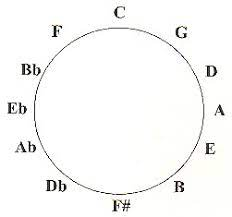
\includegraphics[height=3cm]{circleoffifths}
\end{center}

Our first idea was to begin with a root scale (the starting root scale used is always C major for consistency), and have the following possible paths for the scale to take:

\begin{enumerate}[label=]
    \setlength\itemsep{-1em}
    \item \textit{Very likely:} stay on the same scale (I);
    \item \textit{Likely:} move to the fifth of the current scale (V);
    \item \textit{Unlikely:} move to the fourth of the current scale (IV);
    \item \textit{Very unlikely:} move to the fourth of the fourth of the current scale (VII);
    \item \textit{Very unlikely:} move to the fifth of the fifth of the current scale (II).
\end{enumerate}

However, there was a substantial flaw with this method: it lacked the Markov property! Because each successive case depended on a new root, there was no transition for moving between different states; thus, we had to settle for a new method.

Upon more experimentation, we landed on an abstract system that, storing the starting scale as the \textit{tonal center,} would transition between the following states: 

\begin{enumerate}[label=]
    \setlength\itemsep{-1em}
    \item \textbf{Root:} change to the root;
    \item \textbf{Change:} change to a new scale (50/50 between the fourth and the fifth);
    \item \textbf{New:} update the tonal center to the current scale.
\end{enumerate}

Here is our original Markov chain diagram for these transitions, and the transition matrix with arbitrary probability values:

\begin{center}
    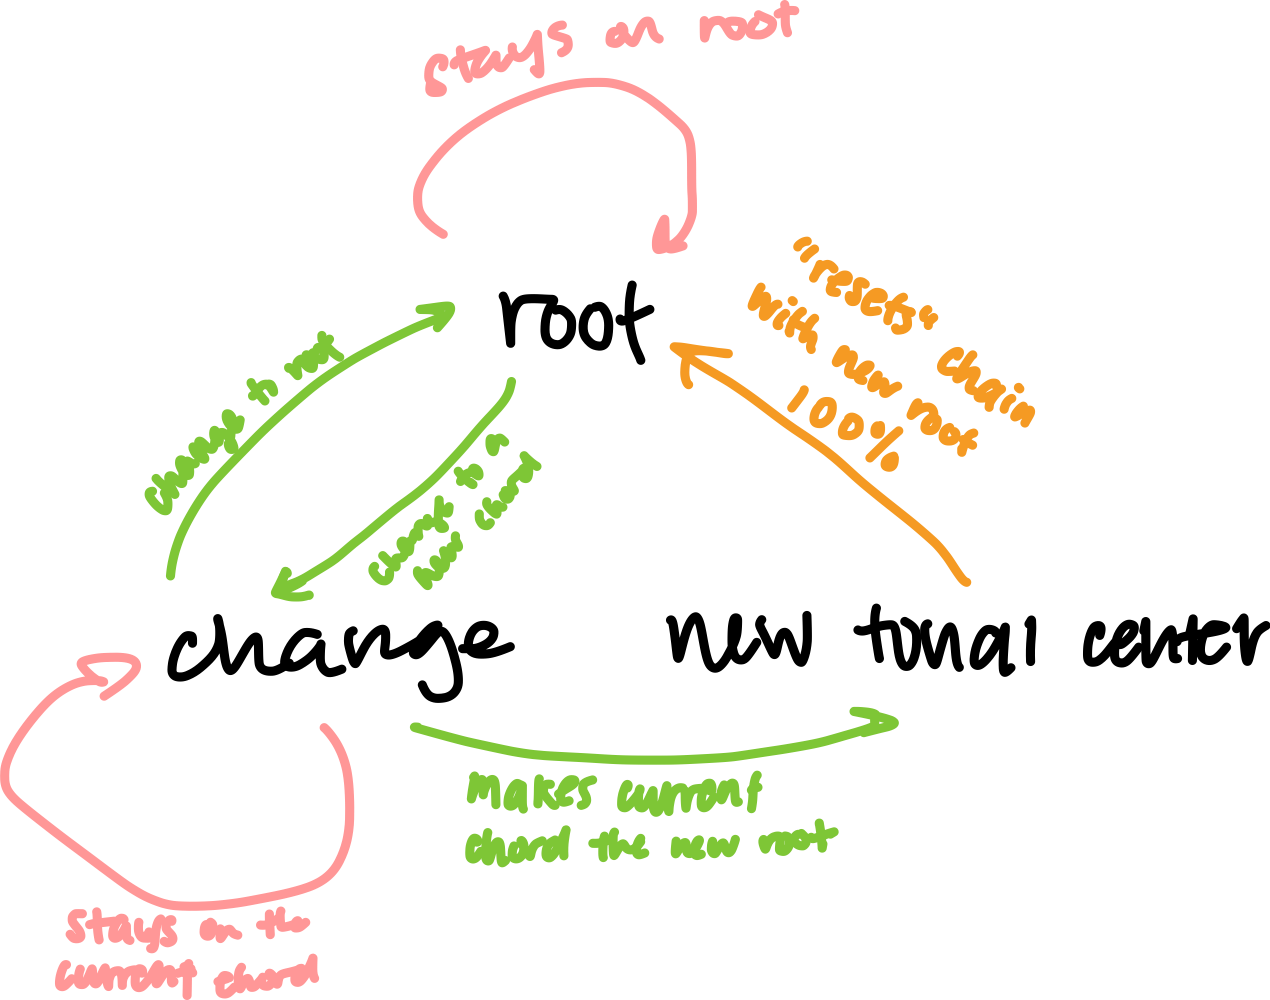
\includegraphics[height=5cm]{diagram}
    \hspace{4em}
    \raisebox{40pt}{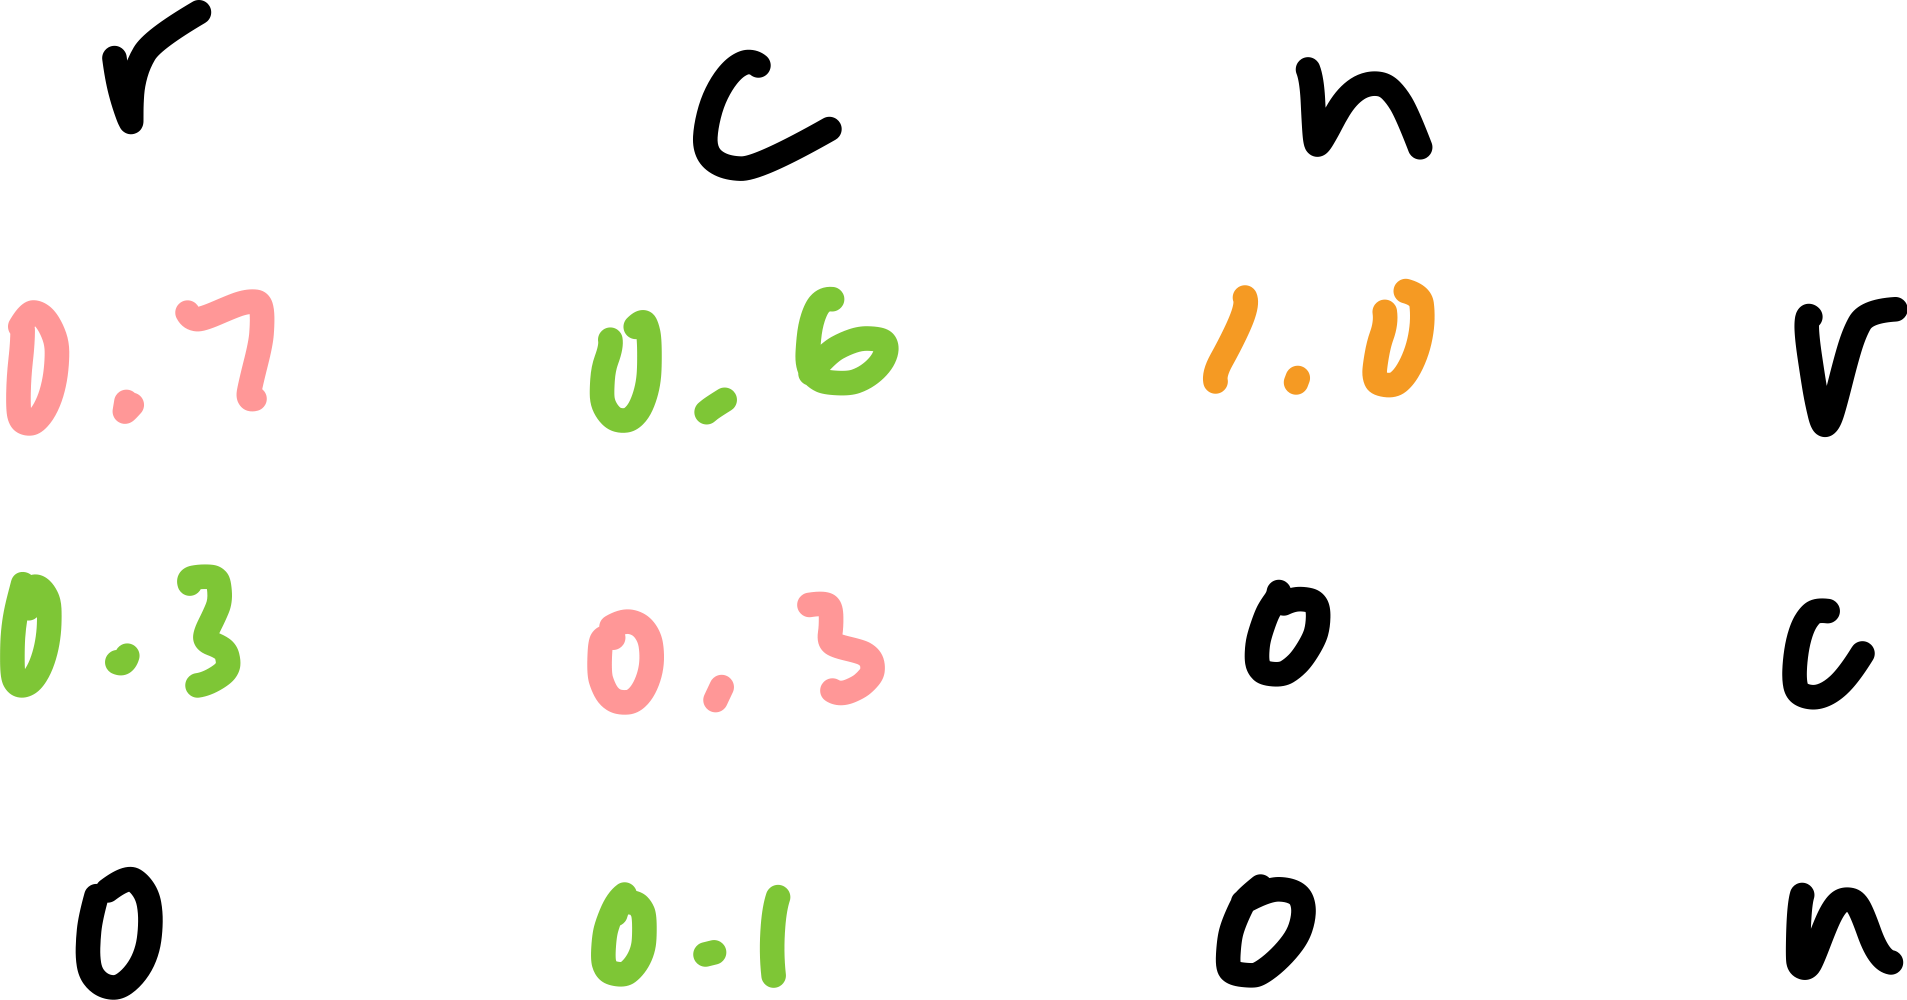
\includegraphics[height=2cm]{originalmatrix}}
\end{center}

To test out this proposition, we used python to simulate this chord progression. With the help of the python libraries \textit{numpy} (complex mathematical calculations) and \textit{musthe} (music elements), we developed a program that would generate a sequence of scale. 

We first defined a Markov chain method that would update our current state (scale) to a new state:

\begin{center}
    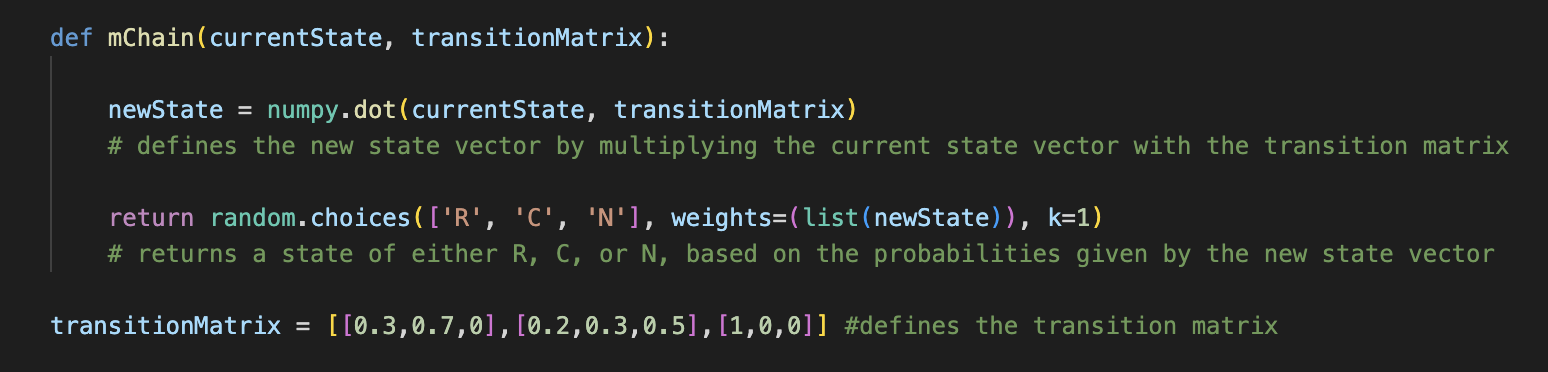
\includegraphics[height=3cm]{mchain}
\end{center}

Note a fundamental difference from the Markov chains described in section 1. Instead of taking the set of probabilities and feeding that back into the transition, we used a weighted randomizer with the given probabilities to actually place the scale definitively into one of the states (thus, our state vector would be comprised of zeroes with one 1), then fed that state vector into the Markov chain again. 

As described earlier, the current state updates the scale and then adds it to a list of scales generated by the program. We ran this code 20 times to create a sequence of 20 scales. 

For the purposes of this project, we used a random note generator to choose four notes in each scale, and then put all the notes in a list. Here is a sample output of the program.

\begin{center}
    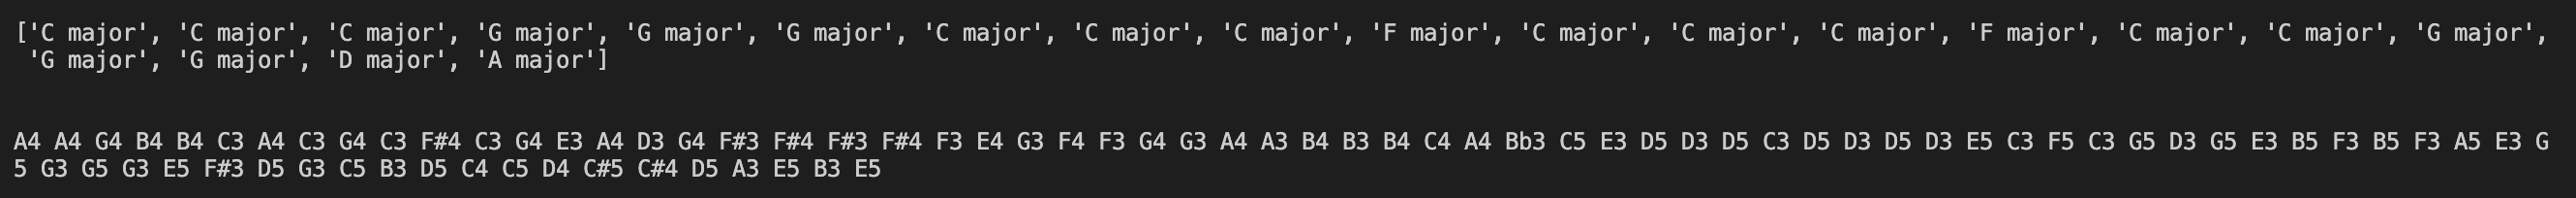
\includegraphics[height=1.2cm]{outputcode}
\end{center}

Feel free to reference the circle of fifths diagram above; looking at the generated chords in the context of the circle of fifths is a good way to understand how the Markov Chains allowed us to introduce randomness and variation without being \textit{too} random.

Now, let's analyze the positive and negative aspects of our R/C/N model.

\textbf{Positives:}
\begin{itemize}
    \item The R/C/N model was good for our purposes of creating a short melody that had controlled variation throughout.
    \item It had a somewhat realistic/plausible cycle through different scales with the movement through fifths and fourths.
    \item The melody sounded pleasant because it was not just completely random; the Markov Chain structure gave realistic probabilities for modulating to new chords.
\end{itemize}

\textbf{Negatives:}
\begin{itemize}
    \item One of the biggest drawbacks of our R/C/N model is that the steady-state property of Markov Chains has no significance in our model. While we could determine the relative probabilities of the steady-state being R, C, or N, there's no way to predict the final chord because that depends on the number of previous R's, C's, and N's. We will elaborate more on this in section four.
    \item Our model only used major scales. Including minor scales or other modes would be an opportunity to introduce more variation.
    \item While the chord generation was not too random, the note generation in most cases was! This is because, if you recall from earlier, our method for choosing the notes from each scale was largely random. This is a place where we could have implemented another Markov Chain to further improve the algorithm.
    \item The probabilities chosen were arbitrary and chosen by us. While this worked for our program, it would be difficult to apply this to analyzing existing work because music isn't normally created with a "R/C/N" method, but rather how likely it is to move to each unique scale from a scale. We will explore projects that worked in this way also in section four.
\end{itemize}

In summary, the R/C/N model worked perfectly for our goal with this project. However, for more complex music generating needs, it would not hold up. Let us now analyze some exiting projects that have implemented some of these possible changes.

\pagebreak

\section{Other Projects and Improvements}

There's a lot of existing literature on this idea. In fact, there are many music-processing and music-creating algorithms dedicated to better understanding these processes such that we can optimize to build very realistic replications of certain composer's style. Of course, most modern machine learning algorithms are based on somewhat black box neural networks that operate akin to a dizzying string of Markov chains.

However, seeing a Markov chain successful in this kind of work is pretty easy to imagine. If we could process lots of data of Bach's work that analyzed the specific probability of each note moving to each note and/or each chord progressing to the next chord, we could build a pretty strong imitation of a typical Bach melody or chord progression. The strength of an AI like we generated above would merely be limited by the ability to take in constructive data and meaningfully spit it back into the matrix. 

This is where we see the R/C/N model fall out of play a bit. It's certainly helpful for our model, but if we want an advanced and replicative process, we would have to build something that's more specific in its knowledge that we can encode. So, we would likely consider something of this model:

\begin{center}
    $A=
    \begin{blockarray}{cccccccccccc}
    C & C\# & D & D\# & E & F & F\# & G & G\# & A & A\# & B \\
        \begin{block}{[cccccccccccc]} 
            x&x&x&x&x&x&x&x&x&x&x&x\\
            x&x&x&x&x&x&x&x&x&x&x&x\\
            &&&&&&\vdots \\ 
        \end{block}
    \end{blockarray}$
\end{center}

With this, there is a great possibility to encode data of the probability of jumping from one note to the next. The difficulty about engineering/tayloring this dataset is how to fit key signatures to a 12 tone system. In similar projects online, we've seen folks normalize the data they receive to force everything into C major: then this matrix becomes a blanket canvas for solfege or assigning scale degrees that are arbitrarily in C major.

There's also the ability to encode this data into a \textbf{second-order markov chain}:

\begin{center}
    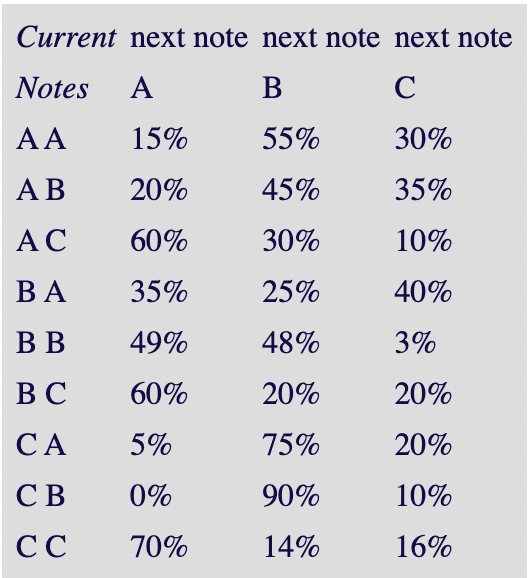
\includegraphics[scale=0.5]{Screen Shot 2022-12-02 at 11.01.07 AM.png}
\end{center}

where the progression of notes would not be based off of discrete notes that came before, but rather the memory of the chain of notes that came before.

With this in mind, melodic motifs and common classical patterns would be very easy to encode. Going to even-higher-order markov chains would assist in building a memory for melodic movement instead of stifling the data by being reliant on discrete instances of notes with no dependence on what came before.

Tying in the bit about steady-states: we can taylor our data set to make sure that it always has ends on a tonic chord. In other words, if we were to normalize the music into c major, almost every piece would end back C. We would have to analyze the matrix, derive its steady state and view its values to see if it somewhat matches the intuition of a composer/music student. This would be one lever through which human intelligence can be a check on the algorithm.

Of course, different genres, composers, and periods would call for VERY different stochastic matrices. However, with enough data intake, developing melodies of these sorts could be rather easy with a strong enough markov chain.

To analyze harmonies, we found several examples online of individuals who built these matrices for various common chords (consider Amin, Fmaj7, etc.) where a user can plug in their own preferance and have a random chord progression to jam out to. Similarly, large research projects have played with rhythm, intensity, and other intelligence heuristics to make the music feel slightly more human.

\section{References}

\begin{enumerate}
    \item Crovella, M. Linear Algebra, geometry, and computation 

    \begin{enumerate}[label=]
    https://www.cs.bu.edu/fac/crovella/cs132-book/L11MarkovChains.html\#steady-state-vectors (accessed Dec 12,  2022). 
    \end{enumerate}
    
    \item Robinson, C. Definition 1. N M M stochastic matrix - Northwestern University 

    \begin{enumerate}[label=]               
    \item https://sites.math.northwestern.edu/clark/354/2002/perron.pdf (accessed Dec 12,  2022). 
    \end{enumerate} 
    
    \item Sapp, C. S. Digital Music Programming II: Markov Chains 

    \begin{enumerate}[label=] 
    \item http://peabody.sapp.org/class/dmp2/lab/markov1/ (accessed Dec 12,  2022). 
    \end{enumerate} 
    
    \item Sekhon, R.; Bloom, R. 10.3: Regular markov chains 

    \begin{enumerate}[label=]     
    \item https://math.libretexts.org/Bookshelves/Applied\_ Mathematics/Applied\_Finite\_Mathematics\_\newline(Sekhon\_and\_Bloom)/1\%3A\_Markov\_Chains/10.03\%3A\_Regular\_Markov\_Chains (accessed Dec 12,  2022).  
    \end{enumerate} 

    \item Unknown Rank of the product of matrices AB is less than or equal to the rank of A 

    \begin{enumerate}[label=] 
    \item https://yutsumura.com/rank-of-the-product-of-matrices-ab-is-less-than-or-equal-to-the-rank-of-a/ (accessed Dec 12,  2022). 
    \end{enumerate}
    
    \item Volchenkov, D.; René Dawn, J. Musical Markov Chains

    \begin{enumerate}[label=]  
    \item https://www.worldscientific.com/doi/pdf/10.1142/S2010194512007829 (accessed Dec 12,  2022). 
    \end{enumerate}
    
\end{enumerate}

\end{document}